\chapter{Applications and Future Improvements}

\section{Applications}

As the purpose of any project or research in engineering is to introduce solutions to real life problems and scenarios, possible V2V applications are provided within the following subsections.

\subsection{Forward collision warning}

The targeted scenarios here are:

\begin{enumerate}
    \item  a car is moving towards a second car in front of it
    \item  a car suddenly stops while having other cars behind it
\end{enumerate}

\begin{figure}[h]
    \centering
    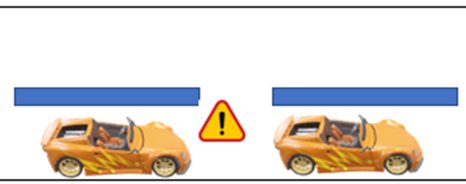
\includegraphics[scale=.7]{figure10/1.png}
    \caption{Forward collision warning}
\end{figure}

In the first scenario the car in the front gets a warning notification while in the second scenario the cars in the rear get the warning notification. This gives the driver enough time to react to avoid collision.
\clearpage
\subsection{Lane change warning}

The working scenario is one car suddenly changes lane, the driver in the targeted lane needs to get a warning notification to avoid a possible accident.\\

\begin{figure}[h]
    \centering
    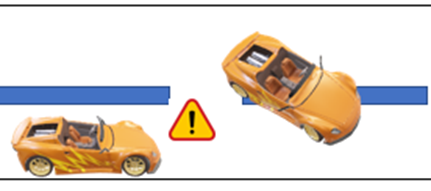
\includegraphics[scale=.7]{figure10/2.png}
    \caption{Lane change warning}
\end{figure}

These two previous applications are near field application and the two cars are in line of sight. In real life, Light Detection and Ranging (LIDAR) could be used for the driver to sense its neighboring vehicles. But due its high cost, it was implemented in this project using ultra sonic sensor.A future upgrade for this project is to use a better detection system as LIDAR for the neighboring vehicles.

\subsection{Blind spot warning}

At a crossroad, it would be hard to notice a fast moving car. This why detection is crucial.

\begin{figure}[h]
    \centering
    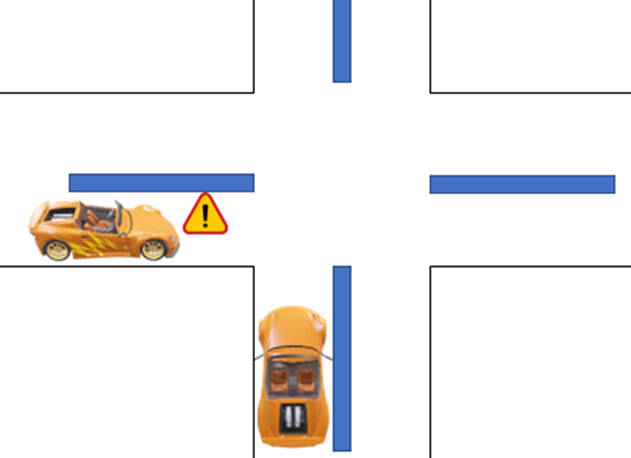
\includegraphics[scale=.5]{figure10/3.png}
    \caption{Motors}
    \label{fig:motors}
\end{figure}

This is near field application, but it is out of sight. To improve the detection of this application, the infrastructure could be used to send data from the streets. If there is a node connected to crossroad gathering information about vehicles in each street, notifying the drivers in case of a speeding car coming from blind spot.
\\

\subsection{Emergency service warning}

Some vehicles require cooperation from other drivers to clear a path for urgent reasons, for example police force, an ambulance, or a firetruck. Sending out a notification to the vehicles in the intended path would help to free a lane for the emergency vehicle to reach its destination as fast as possible.\\

\begin{figure}[h]
    \centering
    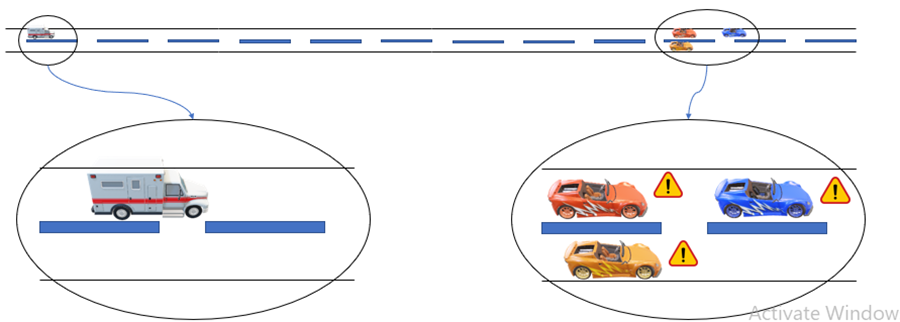
\includegraphics[scale=.5]{figure10/4.png}
    \caption{Emergency service warning}
\end{figure}

This application is far field. The data of the emergency vehicle is known using GPS.\\
A future improvement for this application is to use an algorithm to detect the shortest path for the vehicle and manage the vehicles on this path.

\subsection{Left Turn Assist (LTA) and Right Turn Assist (RTA)}
By identifying stationary or slowly moving cars in front of your car, forward collision warning
systems alert you to the possibility of an impending collision. While you are driving, forward
collision warning uses radar, lasers, or cameras to monitor the road ahead. The technology will
alert you to the danger if there is an oncoming collision utilizing lights, beeps, seat vibrations, or
a combination of these. Additionally, certain systems might tighten your seatbelt and pre-charge
your brakes to help you stop as swiftly as possible.
Forward collision warning systems are rapidly being included into many automobiles, along with
other safety features like automated emergency braking. If you don't apply the brakes quickly
enough to avoid an approaching collision, your car will do it for you if it has automated
emergency braking. Even though autonomous emergency braking might not stop every collision,
the technology might assist reduce the severity of one.
\clearpage
\begin{figure}[h]
    \centering
    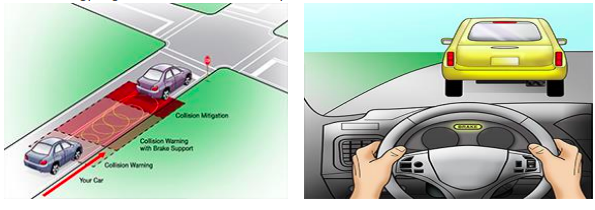
\includegraphics[scale=.5]{figure10/5.png}
    \caption{Left Turn Assist (LTA) and Right Turn Assist (RTA)}
\end{figure}

\subsection{Traffic Management}
V2X will give vehicles an invisible safety net, and the technology will reinforce and expand the
impact of future traffic control strategies. Future management systems will be able to do
without stationary sensors while still having good situational awareness, consider what would
happen if all of the data points from millions of cars were delivered to a single location.
Transportation administrators might modify traffic light timing and shift traffic to make
rush hour flow more smoothly with so much real-time traffic data.

\subsection{Road Safety}
These applications provide information to drivers about a variety of potential risks and
circumstances that are not immediately obvious. They provide support for both time-critical and
less time-critical applications and are in charge of supplying preventative steps to
prevent/minimize hazards or crashes. By connecting your car to the vehicles and roadside
infrastructure around it, V2X technology is about to transform mobility as we know it. With
increased awareness of every nearby vehicle, including those that lie out of sight, your car will
be able to actively reduce the risk of accidents and improve traffic flow.

\section{Future improvement}

Other possible additions or improvements to the project include

\begin{itemize}
    \item Embedding the firmware over the air (FOTA) to add the ability for the driver to update the firmware of the V2V system wireless
    \item Using machine learning to study the behavior of the neighboring vehicles to predict their movements and to digitally flag reckless drivers on the road for other drivers to keep an eye out.
    \item Upgrade the V2V to become V2X. So, the infrastructure is added to the system (V2I), the network is added to the system (V2N),… etc.
\end{itemize}